%%%%%%%%%%%%%%%%%%%%%%%%%%%%%%%%%%%%%%%%%
% Masters/Doctoral Thesis 
% LaTeX Template
% Version 2.5 (27/8/17)
%
% This template was downloaded from:
% http://www.LaTeXTemplates.com
%
% Version 2.x major modifications by:
% Vel (vel@latextemplates.com)
%
% This template is based on a template by:
% Steve Gunn (http://users.ecs.soton.ac.uk/srg/softwaretools/document/templates/)
% Sunil Patel (http://www.sunilpatel.co.uk/thesis-template/)
%
% Template license:
% CC BY-NC-SA 3.0 (http://creativecommons.org/licenses/by-nc-sa/3.0/)
%
%%%%%%%%%%%%%%%%%%%%%%%%%%%%%%%%%%%%%%%%%

%----------------------------------------------------------------------------------------
%	PACKAGES AND OTHER DOCUMENT CONFIGURATIONS
%----------------------------------------------------------------------------------------

\documentclass[
11pt, % The default document font size, options: 10pt, 11pt, 12pt
oneside, % Two side (alternating margins) for binding by default, uncomment to switch to one side
english, % ngerman for German
singlespacing, % Single line spacing, alternatives: onehalfspacing or doublespacing
%draft, % Uncomment to enable draft mode (no pictures, no links, overfull hboxes indicated)
%nolistspacing, % If the document is onehalfspacing or doublespacing, uncomment this to set spacing in lists to single
%liststotoc, % Uncomment to add the list of figures/tables/etc to the table of contents
%toctotoc, % Uncomment to add the main table of contents to the table of contents
%parskip, % Uncomment to add space between paragraphs
%nohyperref, % Uncomment to not load the hyperref package
headsepline, % Uncomment to get a line under the header
%chapterinoneline, % Uncomment to place the chapter title next to the number on one line
%consistentlayout, % Uncomment to change the layout of the declaration, abstract and acknowledgements pages to match the default layout
]{MastersDoctoralThesis} % The class file specifying the document structure

\usepackage[UTF8]{ctex}

\usepackage[utf8]{inputenc} % Required for inputting international characters
\usepackage[T1]{fontenc} % Output font encoding for international characters

\usepackage{mathpazo} % Use the Palatino font by default

\usepackage[backend=bibtex,style=numeric,natbib=true]{biblatex} % Use the bibtex backend with the authoryear citation style (which resembles APA)

\addbibresource{main.bib} % The filename of the bibliography

\usepackage[autostyle=true]{csquotes} % Required to generate language-dependent quotes in the bibliography

\usepackage{url}

%----------------------------------------------------------------------------------------
%	MARGIN SETTINGS
%----------------------------------------------------------------------------------------

\geometry{
	paper=a4paper, % Change to letterpaper for US letter
	inner=2.5cm, % Inner margin
	outer=3.8cm, % Outer margin
	bindingoffset=.5cm, % Binding offset
	top=1.5cm, % Top margin
	bottom=1.5cm, % Bottom margin
	%showframe, % Uncomment to show how the type block is set on the page
}

%----------------------------------------------------------------------------------------
%	THESIS INFORMATION
%----------------------------------------------------------------------------------------

\thesistitle{架构支撑的操作系统安全增强} % Your thesis title, this is used in the title and abstract, print it elsewhere with \ttitle
\supervisor{夏虞斌} % Your supervisor's name, this is used in the title page, print it elsewhere with \supname
\author{杨璧丞、庄浩麒、王帅惟} % Your name, this is used in the title page and abstract, print it elsewhere with \authorname

\university{上海交通大学} % Your university's name and URL, this is used in the title page and abstract, print it elsewhere with \univname

\AtBeginDocument{
\hypersetup{pdftitle=\ttitle} % Set the PDF's title to your title
\hypersetup{pdfauthor=\authorname} % Set the PDF's author to your name
}

\begin{document}

\frontmatter % Use roman page numbering style (i, ii, iii, iv...) for the pre-content pages

\pagestyle{plain} % Default to the plain heading style until the thesis style is called for the body content

%----------------------------------------------------------------------------------------
%	TITLE PAGE
%----------------------------------------------------------------------------------------

\begin{titlepage}
\begin{center}

\vspace*{.06\textheight}
{\scshape\LARGE \univname\par}\vspace{1.5cm} % University name
\textsc{\Large 计算机系统原理课程论文}\\[0.5cm] % Thesis type

\HRule \\[0.4cm] % Horizontal line
{\huge \bfseries \ttitle\par}\vspace{0.4cm} % Thesis title
\HRule \\[1.5cm] % Horizontal line
 
\begin{minipage}[t]{0.4\textwidth}
\begin{flushleft} \large
\emph{作者:}\\
{\authorname} % Author name - remove the \href bracket to remove the link
\end{flushleft}
\end{minipage}
\begin{minipage}[t]{0.4\textwidth}
\begin{flushright} \large
\emph{指导老师:} \\
{\supname} % Supervisor name - remove the \href bracket to remove the link  
\end{flushright}
\end{minipage}\\[12cm]

{\large 2020年12月13日}\\[4cm] % Date

\vfill
\end{center}
\end{titlepage}

%----------------------------------------------------------------------------------------
%	LIST OF CONTENTS/FIGURES/TABLES PAGES
%----------------------------------------------------------------------------------------

\renewcommand{\contentsname}{目录}
\renewcommand{\figurename}{图}
\hypersetup{colorlinks=true,linkcolor=black}

\tableofcontents % Prints the main table of contents

%----------------------------------------------------------------------------------------
%	THESIS CONTENT - CHAPTERS
%----------------------------------------------------------------------------------------

\mainmatter % Begin numeric (1,2,3...) page numbering

\pagestyle{thesis} % Return the page headers back to the "thesis" style

% Include the chapters of the thesis as separate files from the Chapters folder
% Uncomment the lines as you write the chapters

\chapter{总述} % Main chapter title

\label{Chapter1} % Change X to a consecutive number; for referencing this chapter elsewhere, use \ref{ChapterX}

架构支撑的操作系统安全增强
安全,一直是操作系统领域的一个重要方向。
一直以来,研究者们一直致力于保护数据的安全,
保证执行的可靠,
避免代码的 bug。
而由架构支撑的操作系统安全增强,则是其中非常有价值的一个方向。
安全与性能往往是需要权衡的,
加入更多的校验操作,
必然会使程序的运行变得缓慢。
启用硬件架构支撑的安全特性而非纯软件的实现,
可以大大提高安全校验操作的性能,
极大降低提高安全性所带来的开销。

%----------------------------------------------------------------------------------------
\section{硬件扩展的发展}
%----------------------------------------------------------------------------------------
近年来,不断有新的硬件支持的操作系统安全领域的技术出现。
随着技术的不断迭代,硬件扩展的安全技术向着更安全、更方便、更高效不断发展。
例如:
\begin{itemize}
    \item SMEP(Supervisor Mode Execution Prevention) 2011年
    \item SMAP(Supervisor Mode Access Prevention) 2012年
    \item MPX(Memory Protection eXtension)2013年
    \item MPK(Memory Protection Keys)2015年
    \item ARM Pointer Authentication 2017年
    \item Intel Control-flow Enforcement Technology 2018年
\end{itemize}
近年来,TEE 可信执行环境受到了学者们的关注。
在云服务器逐渐被用户接纳的当下,
如何让用户放心大胆的将自己的敏感数据与敏感计算放到云上去运行成为了难题。
TEE 的出现正能回答这个问题。
云服务提供商在自己的硬件设备中创建一个隔离的执行环境,
通过一系列手段使用户相信,在这个环境中执行的应用一定不会被篡改,
数据一定是安全的。
由此使用户敢于将敏感应用云端化,使用云端资源。
而如何构建一个可信执行环境 TEE,不同的硬件架构提供商给出了不同的解决方案。

%--------------------------------------
\subsection{ARM TrustZone}
%--------------------------------------
\paragraph{Normal World 和 Secure World}TrustZone通过TrustedFirmware这一硬件扩展,
将计算机资源划分为安全世界与普通世界。
同时带来与Intel不同的 EL0-EL3 这4个特权等级,
EL3被称为 monitor mode,
只有monitor mode 可以通过运行 ARM Trusted Firmware 来切换普通世界与安全世界。
一台有 TrustZone 的机器,
会经过安全的 bootloader 校验并启动安全世界中的操作系统,
而后,再切换到不可信的普通世界去执行。
%--------------------------------------
\subsection{Graphene-SGX}
%--------------------------------------
\paragraph{Intel SGX}Intel SGX技术通过硬件扩展,提供了 enclave 以及其相关的一些特性。
用户态应用程序可以部分或全部的放入 enclave执行,SGX技术可以保证,
在enclave中执行的程序不会被恶意的操作系统或恶意的Hypervisor攻击,
且数据不会泄露。
\paragraph{Haven}不过,
应用程序适配 SGX是一个挑战。
由于安全性的考虑,
encalve中的程序有一些操作不被允许(例如不能使用syscall),
因此,已有的应用程序想要利用 SGX 带来的安全性,
需要付出大量的重构努力。
OSDI 14 的一个叫 Haven 的工作,提出了带壳执行,证明了
可以将一个已有的二进制应用程序,
通过 libOS 的方式,整个放到enclave中执行。
通过对libOS的API实现进行修改,将底层实现缩小到更少的系统调用,
减少了攻击面。
再对这些与enclave外不受信任的操作系统或 hypervisor 沟通的方法进行校验。
保证出入enclave的控制流的可靠性,并对传输数据进行加密,
已有的应用程序就可以通过把整个二进制放入enclave中的方式利用SGX技术提供的安全性。
\paragraph{Graphene-SGX}Graphene-SGX在 Haven的基础上更进一步,
实现了enclave的安全fork与可信通信,
极大的提高了现有应用利用SGX技术时的可扩展性。
同时,由于硬件的发展,Graphene-SGX的测试还证明了
libOS化的应用程序放入enclave中所带来的开销是可以接受的。

%----------------------------------------------------------------------------------------
\subsection{RISC-V KeyStone}
%----------------------------------------------------------------------------------------
TODO


% Chapter Template

\chapter{TrustZone} % Main chapter title

\label{Chapter2} % Change X to a consecutive number; for referencing this chapter elsewhere, use \ref{ChapterX}

% 思路:
% 1. 介绍TrustZone
% 2. 介绍SANCTUARY
% 3. 小结。

%


%----------------------------------------------------------------------------------------
%	SECTION 1
%----------------------------------------------------------------------------------------

\section{Arm TrustZone}

\subsection{基本介绍} 
TrustZone是一种提高安全性能的硬件架构设计\cite{trustZone-p1}。
它提升了CPU,内存和其他部件的安全能力。
一个支持TrustZone的CPU处理器,可以在四种特权等级下执行指令(EL0-EL3)\cite{trustZone-p2}。
同时TrustZone通过硬件TrustedFirmware(TF)划分了普通世界(Normal World)和安全世界(Secure World)。
EL3拥有最高权限,也被称为monitor mode,可以通过运行ARM Trusted Firmware (TF) 来进行Normal World和Secure World之间的切换。
每个世界中都分别管理自己的地址空间和操作系统\cite{trustZone-p2},
在Secure World中所有App都是运行在可信的操作系统(Trusted OS)上。
在Normal World中所有的App都运行在普通操作系统中。
EL2级别的指令是为每个世界中虚拟机提供的权限,EL1是操作系统内核权限,EL0是用户代码权限。


\begin{figure}
    \centering
    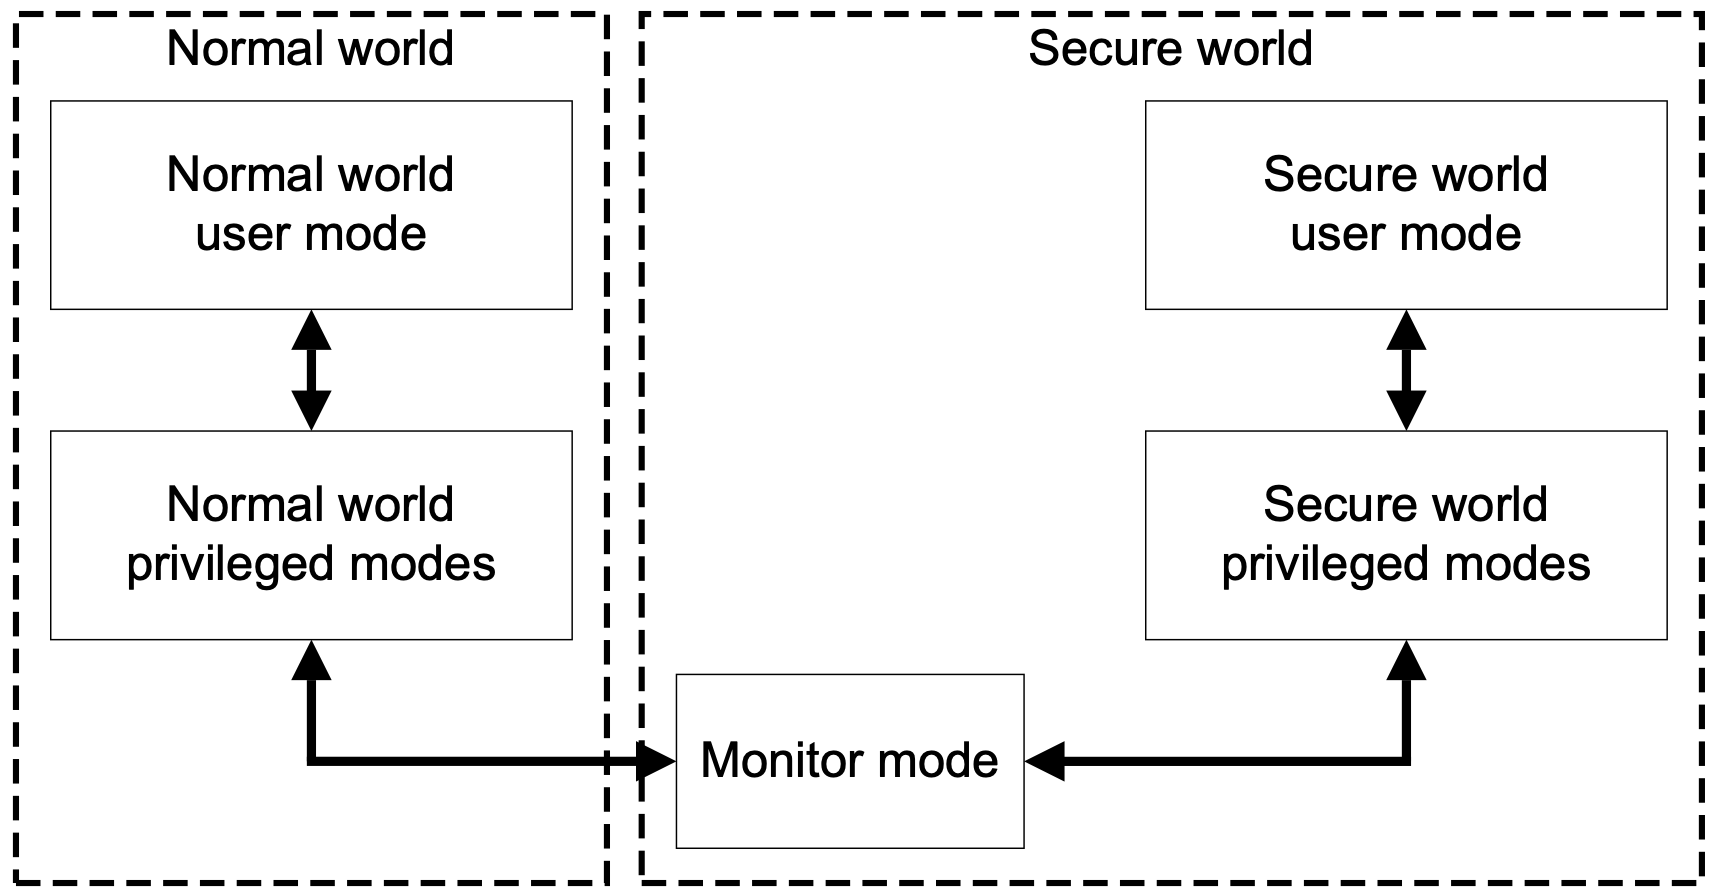
\includegraphics[scale=0.45]{Figures/trustzone/trustzone.png}
    \decoRule
    \caption{TrustZone基本权限设计}
    \label{fig:trustzone}
\end{figure}
(图~\ref{fig:trustzone})展示了TrustZone对Secure World和Normal World的划分\cite{trustZone-p5},
每个CPU可以通过L3级别(monitor mode)的指令secure monitor call (smc)来进行
Secure World和Normal World之间的切换。图中展现了操作系统EL1和应用EL0两种权限,


\subsection {威胁模型} 
原始的TrustZone在威胁模型中作出如下假设:
\begin{itemize}
    \item
    TrustZone的安全模型认为Normal World中的App都是不可信的;
    \item
    在Normal World中运行的OS也是不可信的;
    \item 
    Trusted Firmware是可信的;
    \item
    Secure World中的App,操作系统和boot loader都是可信的。
\end{itemize}

\subsection{安全保证}
首先一个跑在ARM TrustZone的设备会从Secure World中启动,
在初始化完成之后会启动可信操作系统TOS,而boot loader会在执行TOS之前对其进行检查,
确保TOS没有被修改过,接着切换到Normal World启动普通操作系统。
按照这种顺序执行可以保证启动过程的安全,只要boot loader可信就可以保证TOS的完整性。
而在实际场景中终端运营商会通过加锁来防止boot loader被修改。

\begin{figure}
    \centering
    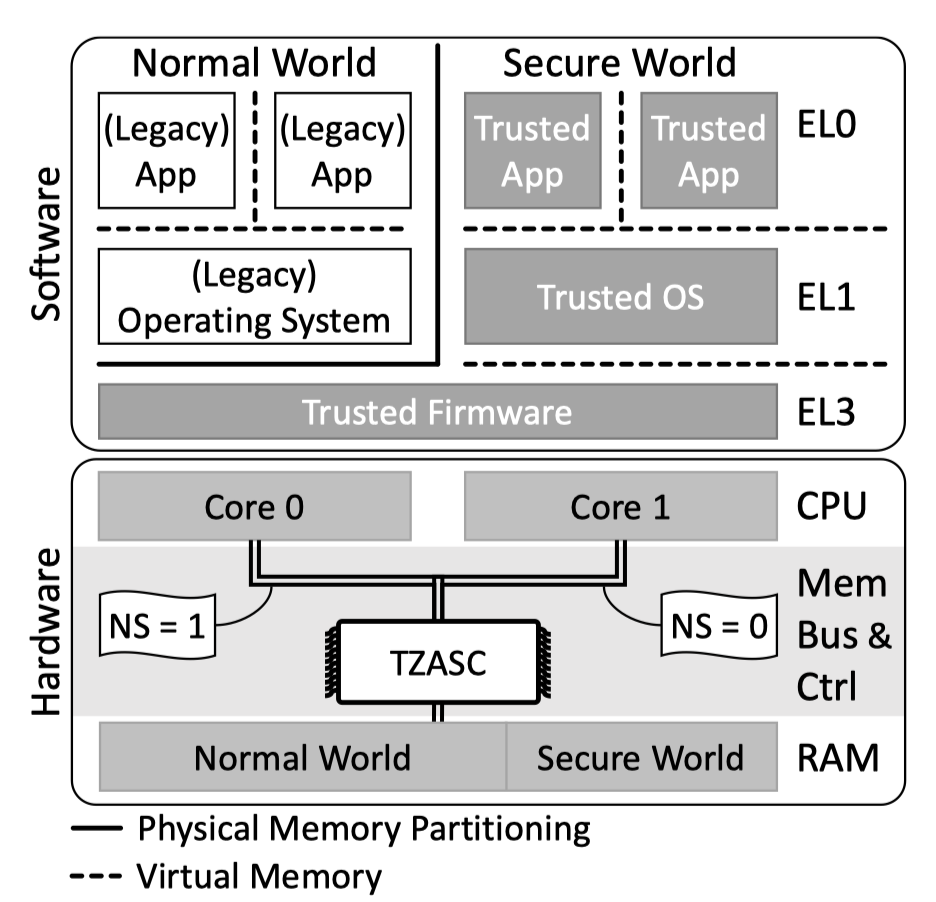
\includegraphics[scale=0.6]{Figures/trustzone/TZASC.png}
    \decoRule
    \caption{TrustZone的TZASC设计}
    \label{fig:tzasc}
\end{figure}
    
其次,TrustZone通过硬件层面上的隔离来防止Secure World中的App和OS被恶意代码攻击\cite{trustZone-p5}。
TrustZone直接将物理内存划分为两部分,其中一部分只能被Secure World访问。
这种物理上的强制隔离主要通过地址空间控制器TrustZone Address Space Controller(TZASC)
来实现。TZASC主要作用于总线和内存之间。
(图~\ref{fig:tzasc})展示了TrustZone Address Space Controller(TZASC)\cite{trustZone-p3}
的基本设计的最原始模式。最原始的TZASC只包含两种内存访问权限non-secure access(NS = 1)
和secure access(NS = 0)。
一个处于secure模式下的CPU可以访问non-secure和secure的内存,
而在non-secure模式下的CPU仅可以访问non-secure的内存。
TZASC现在已经有TZC-380,TZC-400等版本\cite{trustZone-p3}
较新的版本TZC-400,CPU,GPU,DMA等设备都会在硬件上被分配一个bus-master id,
每次访存操作都会附上这个id,这个id可以被用来分配固定物理内存和访问权限,以此做到
物理内存的隔离。
TZASC是使用这种机制来从空间上保证Secure World中的内存不会被其他CPU访问\cite{sanctuary-p1}。



\subsection{不足}
传统的TrustZone存在下列不足:
\begin{itemize}
    \item
    在可信执行环境中,可信的应用(TA)之间的隔离程度较弱,
    一旦一个TA有恶意代码或被攻击,其他应用程序中的敏感数据也会被攻击\cite{trustZone-p6}。
    \item
    在Secure World中的TCB随着App的增多会不断扩展。
    \item 
    一旦黑客可以攻击到Secure World中,收益巨大,使的Secure World成为高价值的攻击目标\cite{sanctuary-p1}。
    \item
    在TrustZone的设计中,一个带有敏感数据(需要被保护)的应用程序(Sensitive App)必须也是一个可以信任的应用程序(Trusted App),
    这样才能够放入Secure World中。
    一个应用程序成为可信应用程序需要运营商和软件开发者相互信任,
    同时需要做大量的检查工作。对于小的开发者来说,
    与vendor建立信任关系并且验证代码是一件费时费力的事情。
    对于vendor来说并不一定就能完全发现可信应用中的恶意代码或者可能被其他人利用的漏洞\cite{sanctuary-p1}。
\end{itemize}


%----------------------------------------------------------------------------------------
%	SECTION 2
%----------------------------------------------------------------------------------------
\section{SANCTUARY}
\subsection{基本介绍}
\paragraph{模型改良}
SANCTUARY\cite{sanctuary-p1}是在TrustZone的基础上为上面的不足提出了合理的解决方案。 
SANCTUARY区分了可信应用程序(Trusted App)和敏感应用程序(Sensitive App),
并把敏感应用程序列入可能有害的威胁模型中。
通在Normal World和Secure World之间设立一个新的区间Sanctuary,如(图~\ref{fig:sanctuary}),
来增加敏感应用程序之间的隔离性。
对于一个运行在Sanctuary中的Sensitive App,Sanctuary可以既保证它免于被入侵,
又可以防止他攻击其他敏感应用程序。
这种设计相比于原来的设计增加了隔离性,减小TCB,
同时一定程度上解决了运营商和应用程序开发者之间协调的问题。

\paragraph{隔离机制}
Sanctuary建立较强的隔离机制,空间上的隔离包括使用TZC-400内存访问控制器,
采用与TrustZone相似的方式强制隔离物理内存,Sanctuary的CPU只能访问自己的物理内存,
不能访问Secure World和Normal World中的内存对于每一个Sanctuary实例单独分配一个独立的CPU资源。
通过避免使用共享缓存,来防止独立内存数据的丢失。
时间上的隔离,包括每次都会从可信的固件(Trusted Firmware)中启动为Sanctuary分配的CPU\cite{trustZone-p1},
在同一时刻内一个Sanctuary环境中只会运行一个应用程序(Sanctuary App),
并且在程序执行结束退出后,会清空其之前使用的内存和缓存。

\paragraph{安全服务}
由于在Sanctuary App执行之前会从没有保护的内存中加载数据。SANCTUARY需要做两种保护。
一种是要保证数据的可靠性,需要验证数据没有被修改过,另一方面SANCTUARY需要防止这些数据
被加载到以一个恶意的Sanctuary App中,因此Sanctuary App本身也需要被验证。对于上面两种
保护,Sanctuary提供了两种安全服务来进行保障。 一种是Remote attestation通过让Sanctuary App
与外部实体建立换一个安全的通道,Sanctuary App通过此通道向提供程序的第三方传输完整性测量数据,
以此保证数据的完整性。第二种是Sealing,这个机制给最初始的Sanctuary App分配一个key,这个
key根据Sanctuary App的哈希值计算得到。Sanctuary App在存储数据时通过这个密钥key进行加密,
读取数据时用这个key进行解密。这样被篡改的Sanctuary App的key会发生变化,因此不能解密得到
正确的数据

\begin{figure}
    \centering
    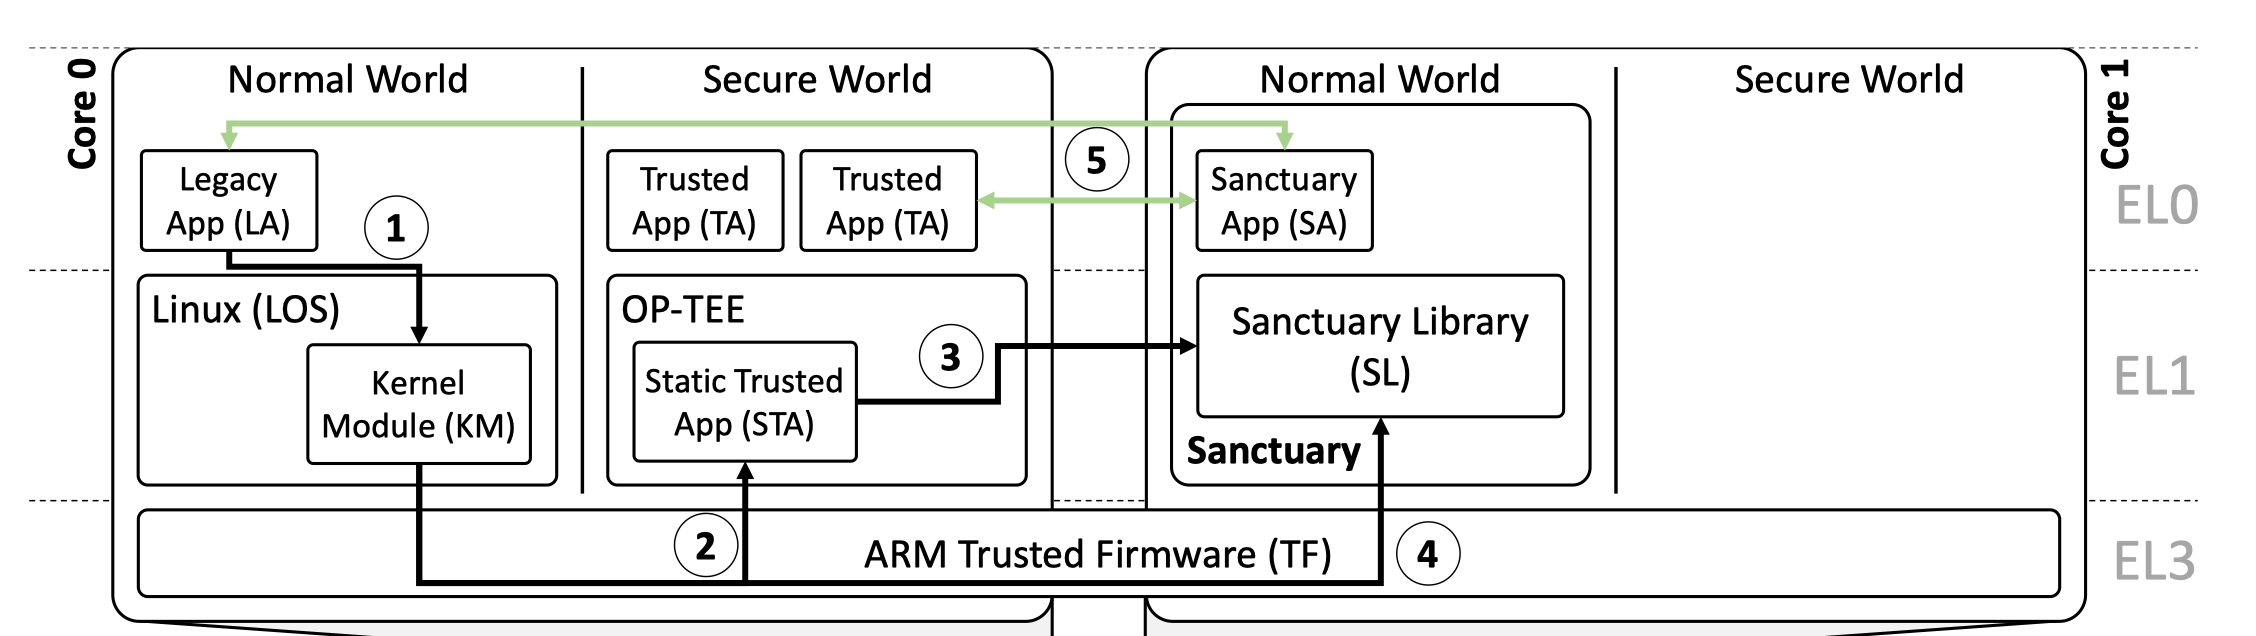
\includegraphics[scale=0.35]{Figures/trustzone/step.png}
    \decoRule
    \caption{Sanctuary 启动步骤}
    \label{fig:step}
\end{figure}

\paragraph{使用方式}
通常,当一个在Normal World中的App需要执行涉及敏感数据的代码时,会调用Normal World
中的Kernal Module(KM)创建一个Sanctuary进行执行。这其中包含五个步骤。如(图~\ref{fig:step})
\begin{itemize}
    \item
    1. 向KM提出执行的Sanctuary App的请求
    \item
    2. KM加载执行Sanctuary必要的运行数据包括Sanctuary library和Sanctuary App,并从
    服务Normal World的CPU中删掉一个,并交给Secure World中的一个专门负责创建相关
    的Trusted App(STA)来操作;
    \item 
    3. STA对Sanctuary App进行一些列的验证操作;
    \item
    4. 验证成功之后,创建Sanctuary实例,并启动;
    \item
    5. 启动后Sanctuary library可以执行敏感代码,并可以与LA和TA进行交流。
    \item
    同时攻击者不进行物理攻击。
\end{itemize}

\begin{figure}
    \centering
    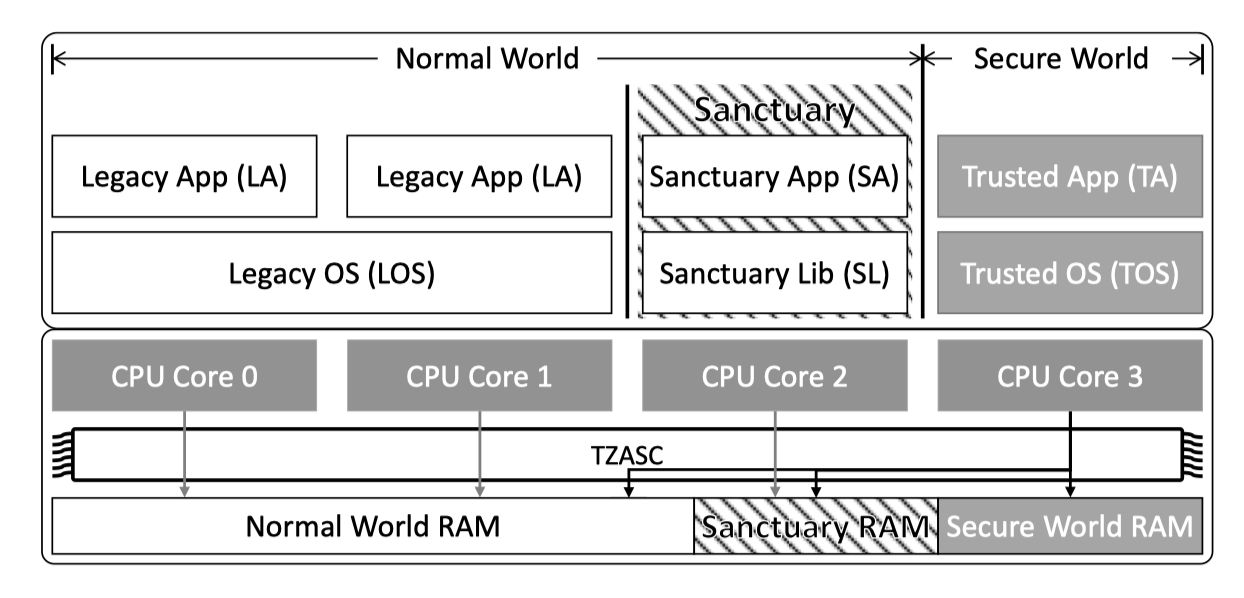
\includegraphics[scale=0.45]{Figures/trustzone/sancutary.png}
    \decoRule
    \caption{SANCTUARY结构图}
    \label{fig:sanctuary}
\end{figure}

\subsection{威胁模型}
SANCTUAR的威胁模型和TrustZone相比进行列继承,细化和延伸:
\begin{itemize}
    \item
    Normal World中的App都是不可信的;
    \item
    在Normal World中运行的OS也是不可信的;
    \item 
    运行在Sanctuary中的敏感应用程序(Sensitive App)也可能是具有恶意的;
    \item
    在Sanctuary假设基于TrustZone的Firmware是可信的;
    \item
    Secure World中的App,操作系统和boot loader都是可信的。
\end{itemize}

\subsection{安全保证}
为了满足威胁模型的要求,既需要保护Sanctuary App免遭攻击,有需要防止有恶意的
Sanctuary App攻击其他部分。接下来从可以攻击的各个角度来详细阐述它的安全保证。

\paragraph{二进制代码完整性}
Sanctuary Library和Sanctuary App的可执行数据都被存在未加密的Normal World的内存中,
SANCTUARY通过本地的验证和远程的验证(Remote attestation)本地验证通过SA最开始存储的
签名来验证,远程验证可以由开发者通过可信通道自己进行验证。如果验证不通过,就拒绝执行
Sanctuary环境也会创建失败,由此保证执行代码的完整性。

\paragraph{代码数据隔离性}
SANCTUARY\cite{trustZone-p1}通过TrustZone自身的特性来保证内存的分离。一旦SANCTUARY内存上锁,除了
SANCTUARY的CPU,其他核均不能对这段数据进行访问。当Sanctuary销毁时,内存数据都会被重置
不会被下一个用此段内存的应用获取到。

\paragraph{存储安全}
SANCTUARY通过key来加密数据,key是通过计算完整SA的哈希值得到的,只有没有被修改过的
Sanctuary\cite{trustZone-p1} App在可以通过key解密得到正确的数据。SANCTUARY运行SA将数据保存到指定的内存中
由此保证数据的可靠性。

\paragraph{缓存攻击}
假设缓存在ARM上由两种,一种时L1,由CPU独享。一种是L2,由多个CPU共享
对于L1Cache的直接攻击\cite{trustZone-p3},SANCTUARY通过只运行在一个核内,且在Sanctuary销毁时,清空缓存来防止。
对与L2Cache的直接攻击\cite{trustZone-p2},可以直接不使用L2缓存,通过outer non-cacheable直接从内存中获取数据,
也可以依靠意见过滤掉带有特定标记的L2缓存。
对于L1Cache的旁路攻击\cite{trustZone-p3},依然可以通过将Sanctuary只运行在一个核上来进行预防。
对于L2Cache的旁路攻击\cite{trustZone-p2},只能通过不使用L2缓存在组织。

\paragraph{恶意的Sanctuary App}
Sanctuary的CPU只能访问自己的内存。并且只运行在单一CPU上,因此不能对Secure World和其他
Sanctuary环境进行攻击。SANCTUARY自身对Sensitive App的隔离性已经很好泛防御恶意的Sanctuary App
对其他Sanctuary App的渗透。

\subsection{模型分析}

\paragraph{性能分析}
如(图~\ref{fig:datacom},图~\ref{fig:setup}和图~\ref{fig:teardown})展示来
SANCTUARY在数据通讯,创建和销毁过程中带来的开销。测试中测试了使用L2缓存和不使用
L2缓存的情况,可以看出通讯和销毁本身的开销不大,禁用L2缓存也不会受到很多影响,而创建
则耗时较多且禁用L2缓存会带来很多的额外开销。总体来讲SANCTUARY的设计的整体开销在一个可以
接受的范围内,但是如果在频繁创建sanctuary的情况下,性能会有所下降。因此让Sanctuary在创建
之后工作一段时间再销毁能提高CPU的利用率。

\begin{figure}
    \centering
    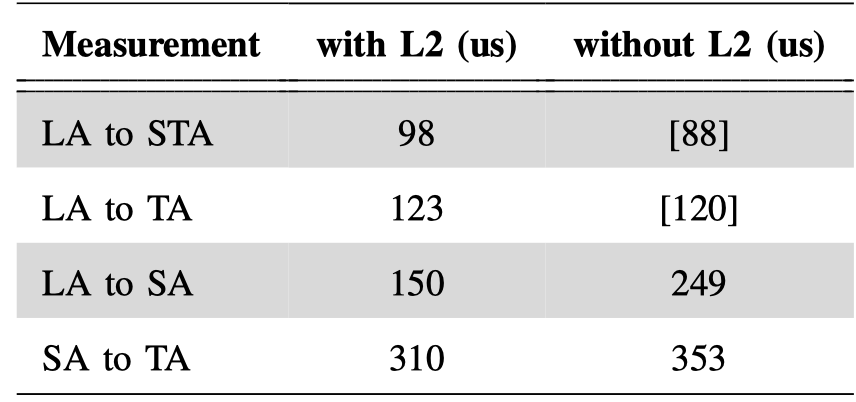
\includegraphics[scale=0.45]{Figures/trustzone/datacom.png}
    \decoRule
    \caption{SANCTUARY通讯性能}
    \label{fig:datacom}
\end{figure}

\begin{figure}
    \centering
    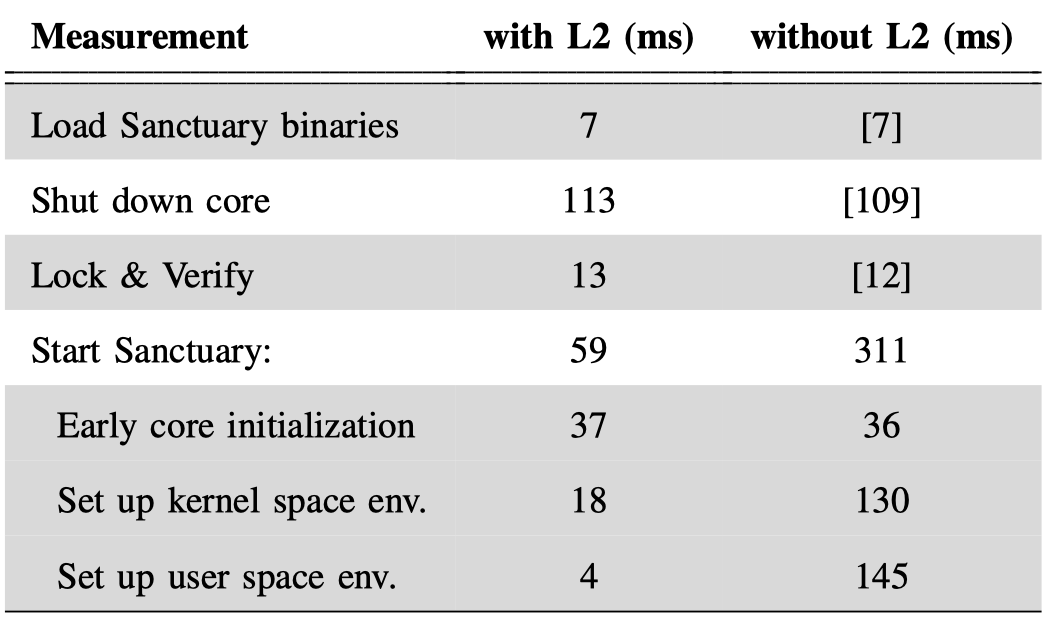
\includegraphics[scale=0.45]{Figures/trustzone/setup.png}
    \decoRule
    \caption{SANCTUARY创建性能}
    \label{fig:setup}
\end{figure}

\begin{figure}
    \centering
    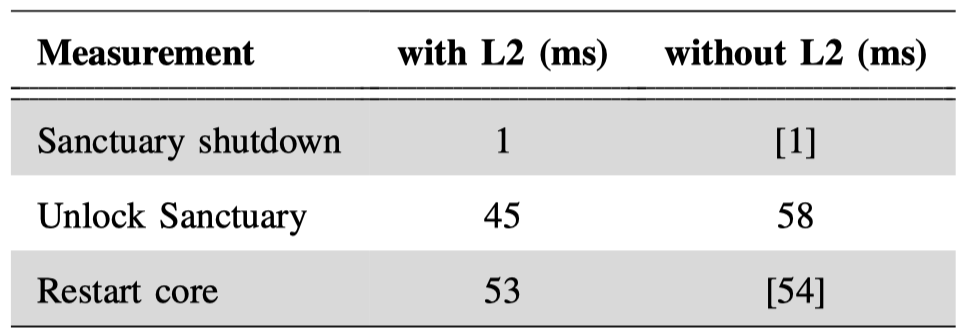
\includegraphics[scale=0.45]{Figures/trustzone/teardown.png}
    \decoRule
    \caption{SANCTUARY销毁性能}
    \label{fig:teardown}
\end{figure}

\paragraph{灵活性分析}
SANCTUARY的设计具有很好的灵活性,不仅不会更改原来的硬件结构,新增和要修改的代码也较少
可以在现有TrustZone的基础上进行直接移植,同时Sanctuary的创建和销毁灵活方便,
可以在实际场景中灵活应用。

\paragraph{可扩展性分析}
可扩展性可以分为从理论和实际两个角度来思考。
从理论和实验上来讲SANCTUARY的设计具有很好的可扩展性,任何一个Normal World的核都可以
被创建成SANCTUARY的CPU,每个Sanctuary也可容易的创建和销毁。
然而在实际终端场景中,一个核的数量终端是有限的,当Sanctuary的数量不断增加,实际可以用
的CPU就会减少,会丧失原本调度的公平性,从而使得整个系统不可用。


\subsection{不足}
\paragraph{恶意使用}
SANCTUARY自身可以有效防止数据被窃取以及获取更高权限的问题。但是其本身不能防止一些恶意
的会让其系统瘫痪的代码。如Sanctuary屏蔽了来自其他地方的中断,因此一个恶意SA可以一直不退出
导致Sanctuary不被销毁,CPU得不到释放,由多个这样的SA足以使系统瘫痪。同时恶意的LA可以通过
不断申请Sanctuary的创建大大降低CPU的利用率。

\paragraph{性能问题}
由于Sanctuary执行的App都是在唯一分配的CPU上执行代码,因此其本身不支持多线程和多核的性能优化。
在一些需要快速响应同时执行敏感数据的场景中,将带来不好的影响。如高清视频的解码。高清的视频流数据
具有版权性,往往需要保护起来,因此在接收和解码时需要放入Sanctuary中执行,而视频观看是一个响应
时间和用户体验挂钩的场景,较慢的解码速度意味着较差的用户体验。Sanctuary的单核设计让解码不能在
多个CPU同时进行,因此可能会影响用户的体验。可以思考在此基础上支持Sanctuary对多核的优化。

%----------------------------------------------------------------------------------------
%	SECTION 4
%----------------------------------------------------------------------------------------

\section{本章小结}

本章主要对TrustZone和系统SANCTUARY进行了介绍和分析,通过说明TrustZone的设计原理和不足,
引出了SANCTUARY的设计和解决方案。说明了SANCTUARY分威胁模型和安全保证。对SANCTUARY的性能
可扩展性以及灵活性进行了分析。最后讨论了SANCTUARY的不足,对于其性能问题给出了具体场景和
未来可以优化的方案。
 
% Chapter Template

\chapter{Graphene-SGX} % Main chapter title

\label{Chapter3} % Change X to a consecutive number; for referencing this chapter elsewhere, use \ref{ChapterX}

\section{Introduction}
Intel SGX技术提供了一系列的硬件特性,帮助保护应用免受操作系统、hypervisor、BIOS和其他软件的伤害。
应用程序可以整个或者部分的放入到enclave中运行,而enclave会有如下功能
\begin{itemize}
    \item 对enclave内的虚拟地址空间的机密性和完整性进行保护。
    \item 限制控制流进入enclave的入口。
    \item 启动时检查内存的内容。
    \item 远程证明。
\end{itemize}

正是因为提供了这些功能,因此用户就可以放心的将他们的敏感应用或者敏感数据放在云服务提供商的enclave中去运行,保证
自己敏感应用的安全性,大大增加了云服务能够服务的对象。
\paragraph{SGX的适配较为困难}为了保证SGX的安全性,在SGX中运行的应用将有一些限制。
比如应用不能在enclave中调用syscall,而是通过一层shielding code去访问syscall,通过sheld层,syscall的结果
在返回给应用之前会被验证,保证结果的安全可靠,防止host的操作系统攻击enclave中的应用。因此,普遍认为
应用程序适配SGX需要付出大量的努力。
前人的工作 Haven \cite{186173}展示了可以利用一个 library OS 把没有修改过的应用放到SGX中去。
但是这需要付出性能上的 overhead 和TCB的扩大的代价。
不过,Graphene-SGX验证了实际上利用library OS带来的overhead并没有前人所称的那么大,
利用Graphene-SGX可以快速的把现有的应用放到enclave中去运行,并且没有很大的开销。

\paragraph{Graphene-SGX并不是最优的}
Graphene-SGX这一工作的目的并不是为了追求更好的SGX技术利用性能,
而是为了把已有工作更快的部署到enclave中去。
因此,虽然有很多方法可以提升enclave代码中的性能,
降低代码的TCB,
但是enclave都暂未采用,因为这些优化会令应用的适配更加复杂。



\section{威胁模型}
Graphene-SGX 的威胁模型与典型的 SGX 应用的威胁模型类似。
下列的组件是不被信任的:
\begin{itemize}
    \item [1)] 
    除CPU之外的硬件。
    \item [2)]
    操作系统、hypervisor和其他的系统软件。
    \item [3)]
    在enclave之外跟其他enclave之内运行的应用程序。
    \item [4)]
    同一应用程序的enclave之外的部分。
\end{itemize}   
\paragraph{}
Graphene-SGX只信任CPU,还有enclave内部的代码(shielding module、bootloader)。
还必须信任Intel的SGX SDK中的aesmd工具,该工具验证enclave签名中的属性并批准enclave的创建。
这是现在利用SGX技术的所有工作都必须信任的。
除此之外,虽然Graphene-SGX使用且仅使用了Intel SGX SDK 中的驱动程序,但是并不信任他。

\section{保证的安全性质和能够防御的一些具体攻击}
\begin{figure}
    \centering
    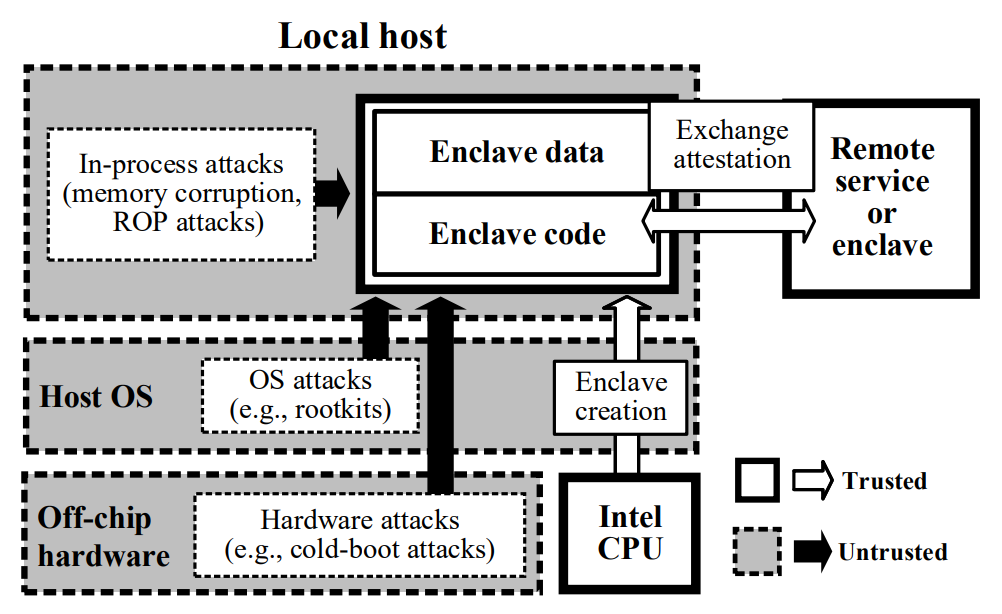
\includegraphics[scale=0.35]{Figures/SGX/threatmodel.png}
    \decoRule
    \caption{Graphene-SGX的威胁模型}
    \label{fig:Graphene}
\end{figure}

\subsection{保证的安全性质}
\paragraph{继承自SGX的性质}
Graphene-SGX 是对SGX技术的应用,因此,Intel SGX 技术提供的保护也被完全的继承。
1)对enclave内的虚拟地址空间的机密性和完整性进行保护。
2)限制控制流进入enclave的入口。
3)启动时检查内存的内容。
4)连接Intel服务器进行远程证明

\paragraph{Graphene-SGX提供的特性}
除此之外,Graphene-SGX还提供了很多其他安全性质。
例如:
\begin{itemize}
    \item 通过本地验证证明两个本地enclave是安全的。
    \item 在两个安全的本地enclave之间搭建安全通信。
    \item 提供安全的fork机制创建一个新的enclave。
\end{itemize}

\subsection{能够防御的具体攻击}
\begin{itemize}
    \item [1)]\textbf{来自host上其他进程的攻击} memory corruption,ROP attack
    \item [2)]\textbf{自host OS 的攻击}rootkits
    \item [3)]\textbf{来自硬件的攻击}cold-boot attacks
\end{itemize}

\section{性能、可扩展性(scalability)、灵活性等分析}
\begin{figure}
    \centering
    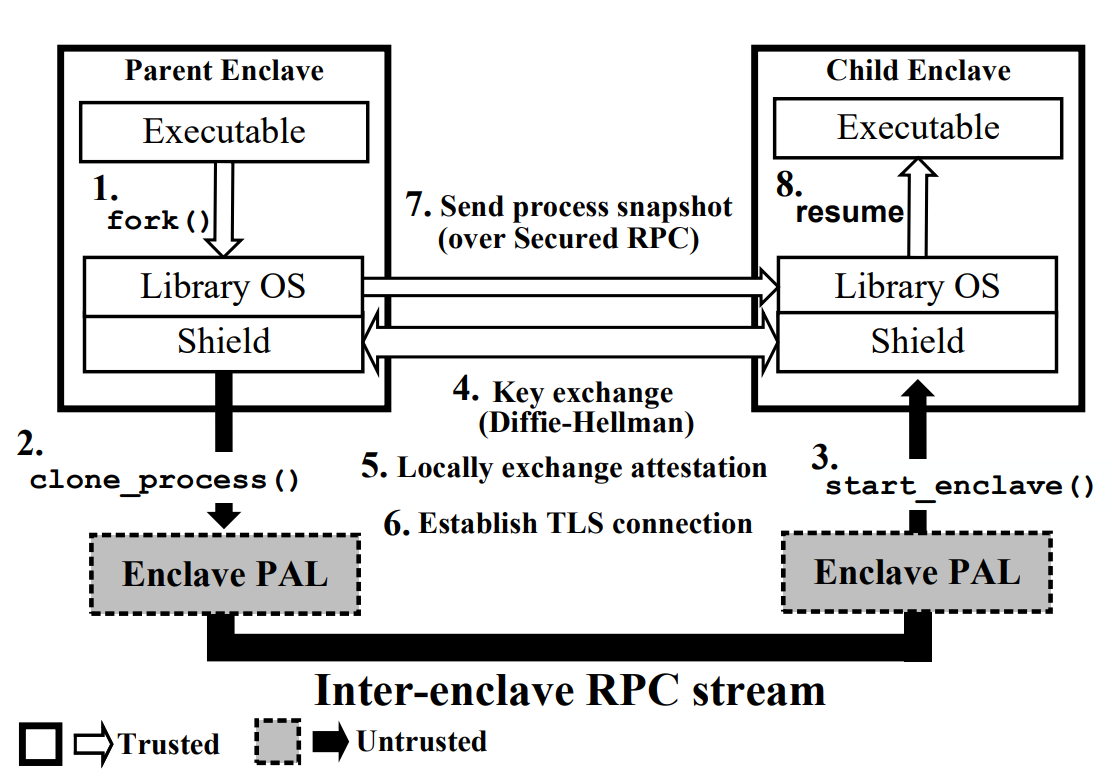
\includegraphics[scale=0.35]{Figures/SGX/enclavescale.png}
    \decoRule
    \caption{encalve的fork与加密通信}
    \label{fig:enclavescale}
\end{figure}
\subsection{灵活性和可扩展性}
由于Graphene-SGX可以直接在enclave上运行没有经过修改的Linux程序,因此,通过Graphene-SGX可以快速的
帮助现有应用利用到SGX的enclave这一特性,提高已有应用的安全性,而同时不需要付出太大的开发成本。

在可扩展性方面,Graphene-SGX还提供了enclave的fork操作如图\ref{fig:enclavescale}所示,用户可以简单的通过一个enclave环境,
fork出一个新的子enclave环境。
同时 Graphene-SGX 还提供了两个enclave之间的加密通信,互相验证的功能。
因此,多进程的应用程序可以有效的保留多进程抽象的同时利用SGX技术带来的安全保证。


\subsection{性能分析}
\begin{figure}[]
    \centering
    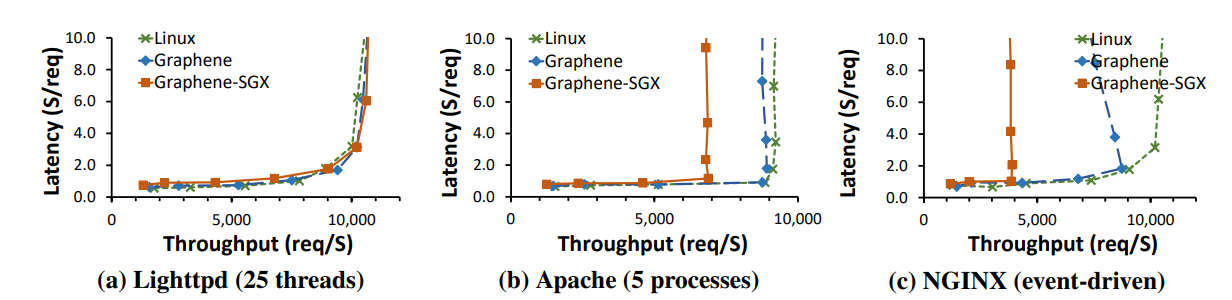
\includegraphics[width=1\textwidth]{1.png}    
    \caption{三种应用(Lighttpd、Apache、NGINX)
    分别在Linux、Graphene、Graphene-SGX环境下的性能表现}
    \label{23333}
\end{figure}
图\ref{23333}展示了Graphene-SGX的性能分析。
可以从途中看出,对轻量级的网站服务应用\textbf{Lighttpd}来说,
Graphene-SGX对性能的影响不大。对\textbf{Apache}来说,由于Apache服务器有多个worker,
每个worker在一个enclave环境中,因此worker之间的通信,请求的传输,
都需要用到enclave之间的加密通信,会消耗很大的性能。
因此,如果不用SGX的话,单独的Graphenen技术并不会带来多少的overhead,但是如果要保证安全性,
对性能就会产生影响。
\textbf{NGINZ}服务器由事件驱动,因此Graphene的shielding 层对数据的检查会有overhead,因此性能更差。

不过,由于Graphene-SGX主要致力于将应用快速的部署到SGX提供的enclave中去,所以很多性能优化的工作都未集成。
在已有快速部署已有应用这一特性的前提下,Graphene-SGX的性能对先前工作来说也是很有竞争力的。


\section{不足}
\paragraph{无法防御一些攻击}
Denial of service,sidechannels,controlled-channel attacks这些攻击是目前所有的 SGX 平台都难以防御的,Graphene-SGX同样无法处理。
\paragraph{不能保证可用性}
像其他的利用SGX的平台一样,
Graphene-SGX可以保证代码在enclave内部的安全执行,
但是无法保证enclave本身的可用性。
例如,恶意的操作系统可以一直不返回到enclave中,或者在某些需要等待的操作中提前返回enclave使受保护的代码执行超出预期。

\section{本章小结}
本章主要对 Graphene-SGX 进行了分析。Graphene-SGX 是一个帮助现有应用,
快速利用 Intel SGX 技术保护数据与正确执行的工作。
与其前作 Haven(OSDI14) 相比,Graphene-SGX 得益于SGX硬件的进步,
在真实的硬件上评估了shield-exection 的性能,
论证了将整个应用二进制通过libOS的方式直接放入 enclave中执行的可行性。
同时实现了 enclave 的安全fork等操作,
同时实现了 encalve之间的加密通信。
通过不断的努力,将现有应用不加修改的放入enclave中执行已经成为了可能,
已有应用通过 libOS 能快速的获得 SGX技术提供的数据与执行的安全保障。
%----------------------------------------------------------------------------------------
%	SECTION 1
%----------------------------------------------------------------------------------------

% Chapter Template

\chapter{RISC-V KeyStone} % Main chapter title

\label{Chapter4} % Change X to a consecutive number; for referencing this chapter elsewhere, use \ref{ChapterX}

\section{Introduction}
Keystone基于RISCV指令集架构,是第一个构建定制TEE的开源框架。Keystone使用了基于硬件的简单抽象,如内存隔离和在不可信部件(如OS)之下的可编程层。Keystone从这些抽象中构建可重用的TEE核心原语,同时允许特定于平台的修改和应用程序特性。

\section{威胁模型}
Keystone信任以下部分:
\begin{itemize}
	\item [1)]
	PMP (Physical Memory Protection)
	\item [2)]
	信任RISC-V架构无BUG
	\item [3)]
	Keystone用户只在Secure Monitor被验证后信任它
	\item [4)]
	Secure Monitor只信任硬件
	\item [5)]
	Root of Trust信任Secure Monitor
	\item [6)]
	Enclave app信任Secure Monitor和Root of Trust
\end{itemize}
Keystone假设有以下这些攻击者:
\begin{itemize}
	\item [1)]
	物理攻击者可以截获、修改或重放离开chip package的信号。Keystone假设物理攻击者不会影响chip package内的组件。
	\item [2)]
	软件攻击者可以控制主机应用程序、不受信任的操作系统、网络通信、启动恶意的enclave、任意修改任何未受TEE保护的内存,以及添加/删除/重放enclave消息。
	\item [3)]
	侧通道攻击者通过cache side-channel、timing side-channel或control channel被动地观察可信组件和不可信组件之间的交互,从而收集信息。
	\item [4)]	
	拒绝服务攻击者可以攻击enclave或主机OS。Keystone不防御这些攻击,因为OS可以在任何时候拒绝为用户应用程序提供服务。
\end{itemize}

\section{保证的安全性质和能够防御的一些具体攻击}
\subsection{安全保证}
\paragraph{内存隔离}
Keystone使用RISC-V架构提供的PMP (Physical Memory Protection) 来进行内存保护。
PMP通过定义相应的PMP region来限制User-mode和Supervisor-mode的内存访问。
RISC-V架构拥有16个pmpaddr寄存器和4个pmpcfg寄存器,pmpaddr寄存器用来存放相应region的地址(物理地址),
pmpcfg寄存器用来定义访存权限、region区间对齐方式以及是否锁定该region.
\paragraph{通过Secure Monitor加强内存隔离}
在RISC-V架构中,存在Machine-mode这一高于Supervisor-mode的特权级,Secure Monitor便运行在这一模式。
在CPU将控制转移给enclave时,Secure Monitor会enable当前要执行的enclave的PMP permission bits. 
并disable OS拥有的所有PMP的permission bits,以此来保证enclave只能访问自己的region.
在CPU从enclave退出时,Secure Monitor会disable enclave的PMP permission bits,
并enable OS的PMP permission bits.
Secure Monitor的这些操作,在更高的权限级(M-mode)保证了PMP的安全性。

\subsection{能够预防的具体攻击}
对于Enclave的保护:
\begin{itemize}
	\item [1)]
	\textbf{Mapping Attacks} Enclave运行在可信的RT(runtime)之上,故RT本身不会去做恶意的mapping. 并且OS给enclave配的页表会经过SM的检查。
	\item [2)]
	\textbf{Syscall Tampering Attaks} Enclave调用syscall可能会受到Syscall Tampering Attack,Keystone可以将已有的防御措施(如SCONE、Graphene等)作为Plugin来防御这些攻击。
	\item [3)]
	\textbf{Side-channel Attacks} Keystone提供cache partitioning,可以防止Side-channel Attacks.
\end{itemize}

\section{性能、可扩展性(scalability)、灵活性等分析}
\subsection{性能}
\begin{figure}[]
    \centering
    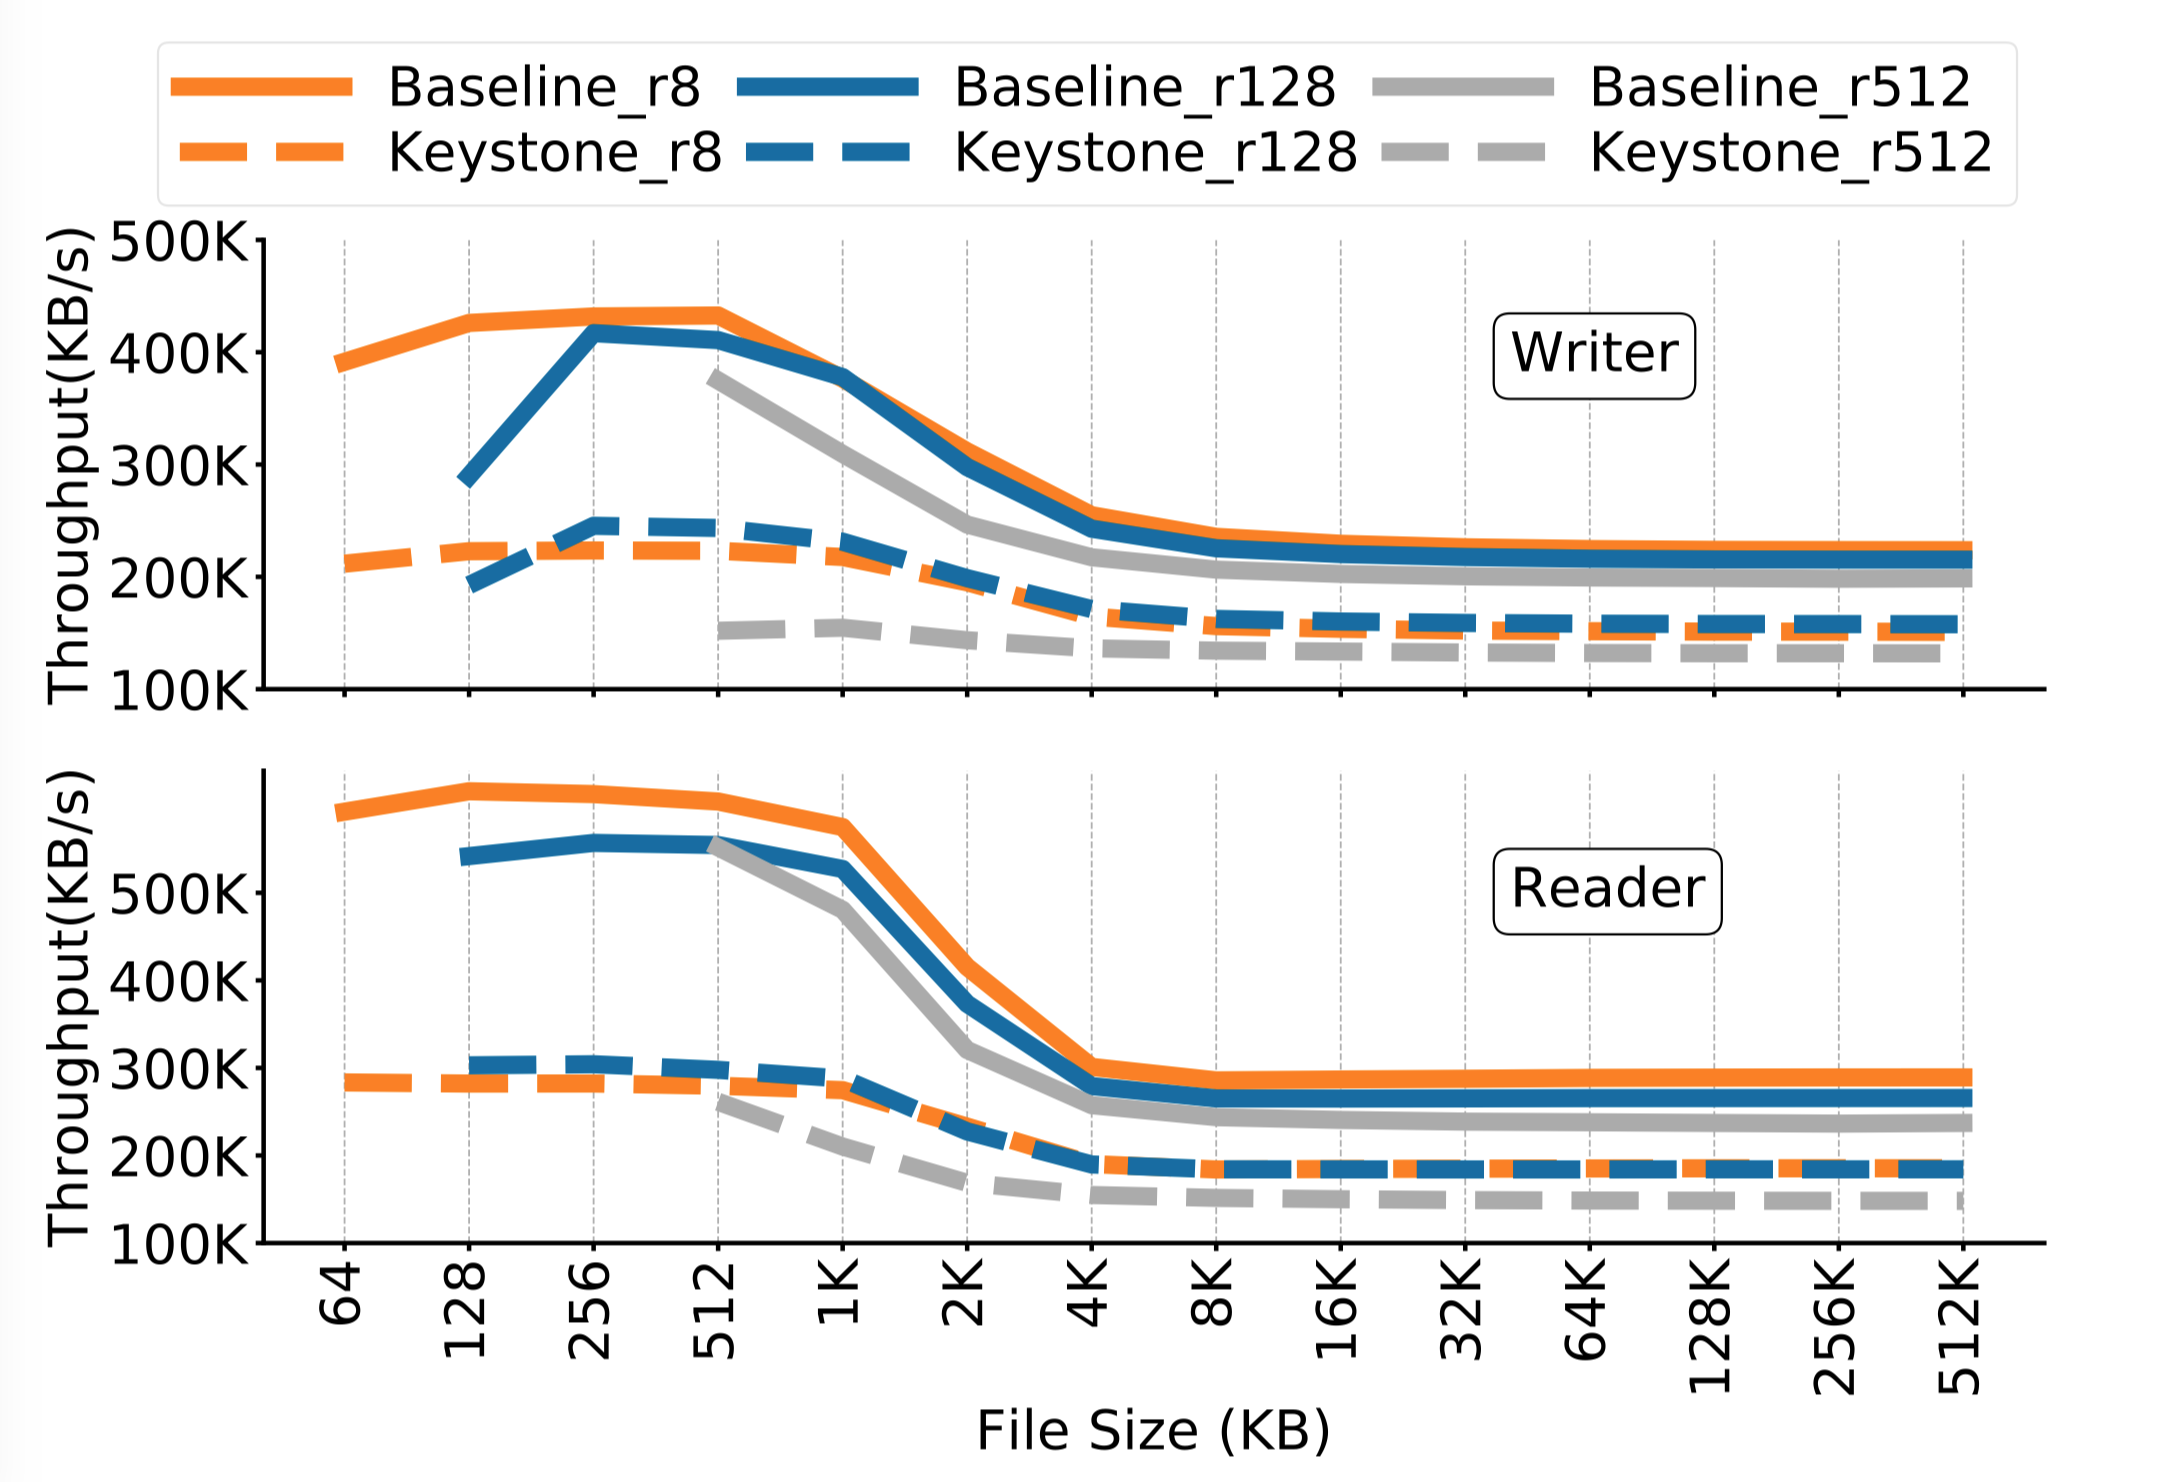
\includegraphics[width=1\textwidth]{memory-eval.png}    
    \caption{Keystone和baseline运行IOZone benchmark}
\end{figure}
上图是Keystone和baseline(linux)运行RV8 benchmark,可以看到,Keystone的访存性能大概在baseline的一半左右,考虑到其运行在enclave内,这个overhead还能接受。
\begin{figure}[]
    \centering
    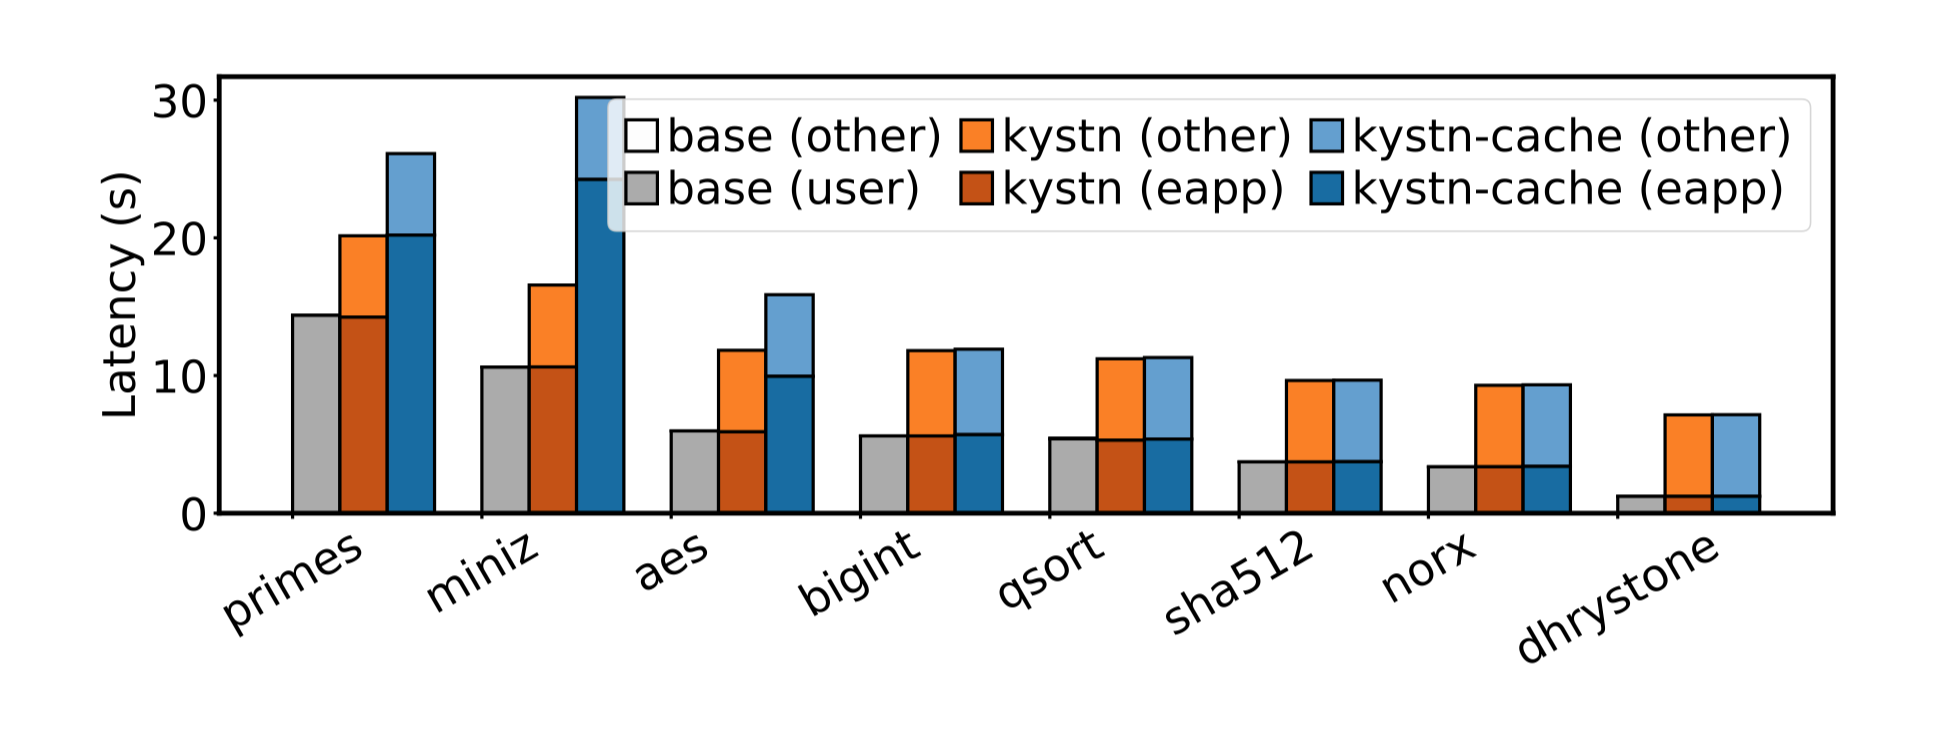
\includegraphics[width=1\textwidth]{calculation-eval.png}    
    \caption{Keystone和baseline运行RV8 benchmark}
\end{figure}
上图是Keystone和baseline(linux)运行IOZone benchmark,可以看到,由于workload本身在enclave内,Keystone并没有增加计算的latency.
\subsection{可扩展性和灵活性}
由于Keystone是基于RISC-V的开源框架,所以其可扩展性和灵活性都颇佳。
首先,由于RISC-V架构非常轻便,开发者可以很方便的自己修改硬件特性,Keystone可以部署在支持RISC-V架构的平台上。
其次,使用PMP做内存隔离非常灵活。在RISC-V里一共有16个PMP寄存器,可以灵活的给多个enclave分配region。不会像SGX那样,对EPC的大小有限制,也不要求一个enclave的物理地址空间必须要连续。
最后,Keystone支持自定义的Plugin选择,可以让开发者自由选择需要的安全特性,使其可扩展性和灵活性更上一个台阶。

\section{不足}
\begin{itemize}
	\item [1)]
	Keystone PMP寄存器的数量只有16个,
	还要分配一部分来保护Secure Monitor以及供OS正常访存使用。
	这样一来,可以用来给enclave使用的PMP寄存器就更少了。
	\item [2)]
	Keystone不能防御DoS攻击,因为其还是需要一个正常运行的OS(配页表、syscall等),恶意的OS可以拒绝服务用户。而Keystone没有修改OS,所以不能防御DoS攻击。
\end{itemize}

\section{本章小结}
本章从Keystone的威胁模型出发,详细介绍了其提供的安全保障。
并且举例介绍了keystone可以防御的具体攻击。
本章其后分析了keystone的性能,并且就其可扩展性与灵活性做了分析。
最后,本章简述了keystone的不足之处。
 
\label{Chapter5} % Change X to a consecutive number; for referencing this chapter elsewhere, use \ref{ChapterX}
\chapter{扩展方案} % Main chapter title
\section{目标问题}
上述提到给予RISC-V中PMP设计的KeyStone存在PMP寄存器不足的问题,
如(图~\ref{fig:pmpcfg}), 在RV64的模式下有2个pmpcfg寄存器pmpcfg0和pmpcfg2,
包含了可以指明解析方案的16个8个bits组成的pmpxcfg寄存器,即pmp0cfg-pmp15cfg。
在一些场景下仅仅这16个权限寄存器可能并不足够。为了在不改变原始硬件的情况下,
增加可用的PMP寄存器范围,可以给出PMP寄存器的扩展方案。

\begin{figure}
    \centering
    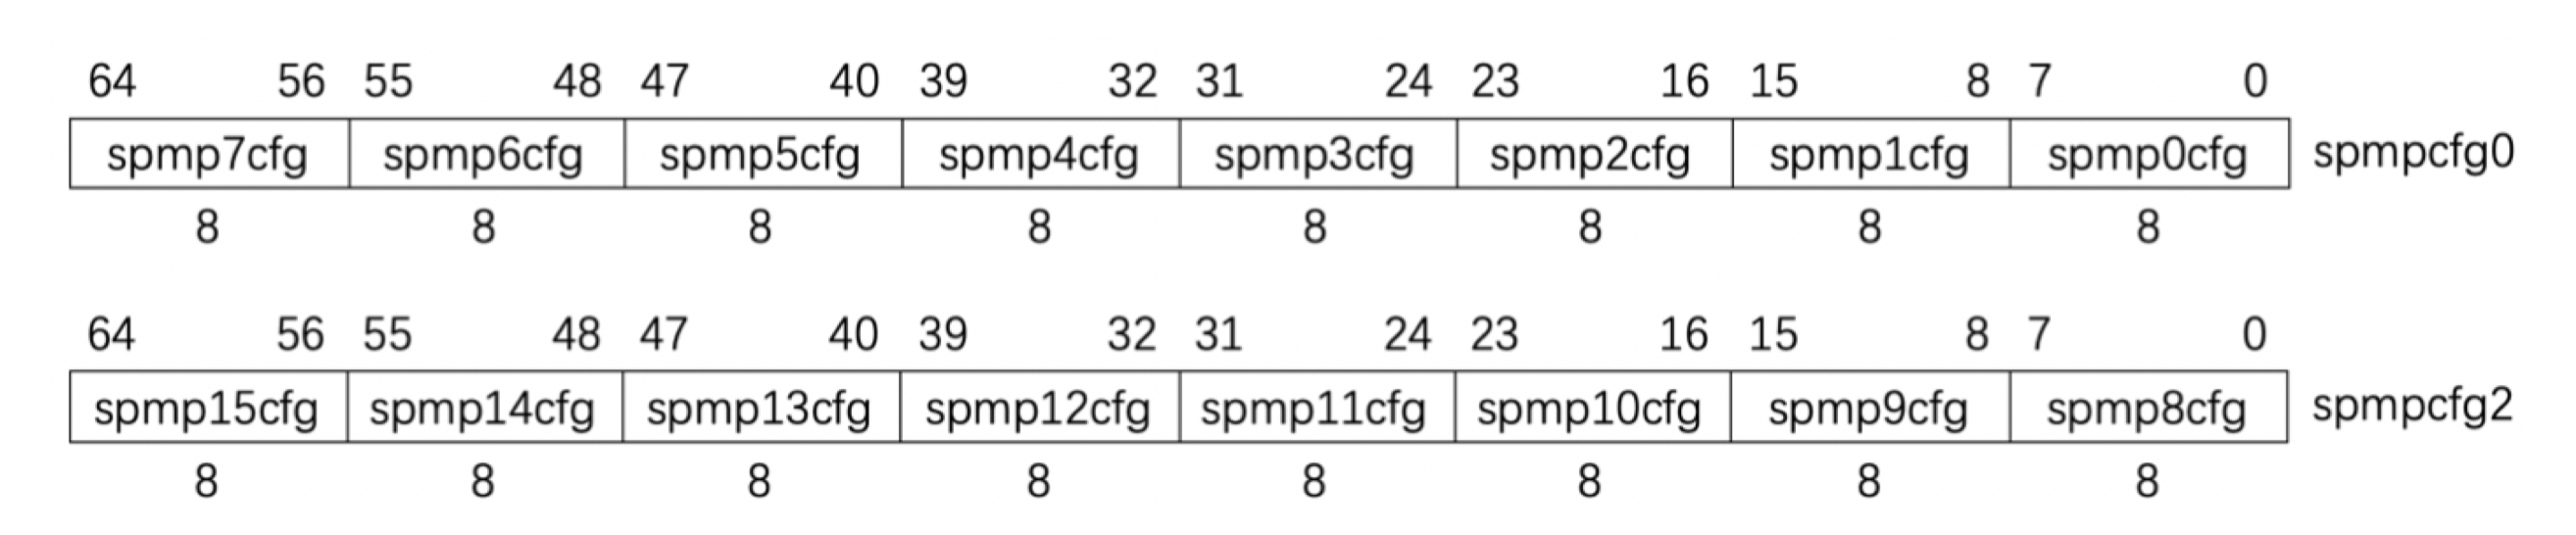
\includegraphics[scale=0.30]{Figures/extend/pmpcfg.png}
    \decoRule
    \caption{pmpcfg寄存器}
    \label{fig:pmpcfg}
\end{figure}

\begin{figure}
    \centering
    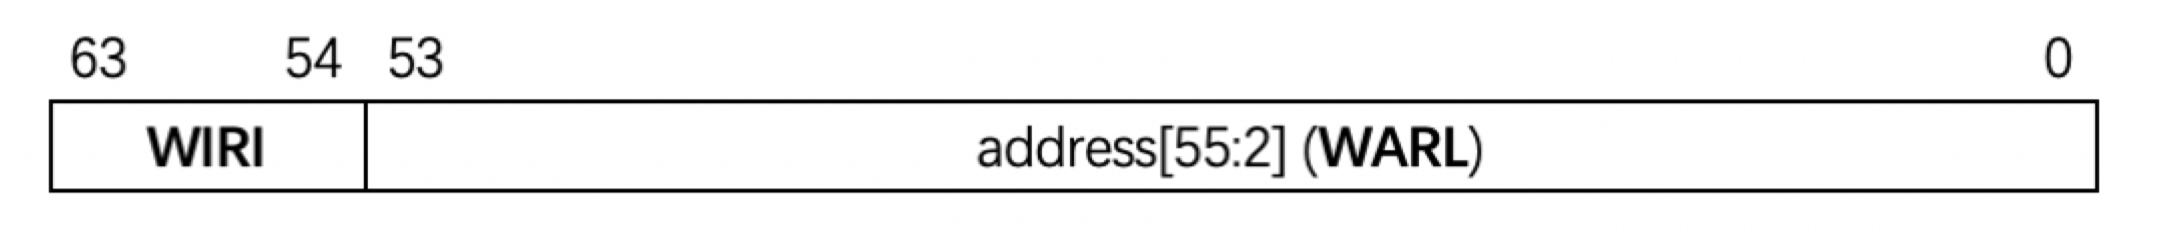
\includegraphics[scale=0.30]{Figures/extend/addrformat.png}
    \decoRule
    \caption{地址寄存器格式}
    \label{fig:addrformat}
\end{figure}

\section{扩展思路}
原始的PMP是通过Monitor来配置Machine Code用来保护Monitor最基本的物理地址空间。
为了扩大保护的范围,可以考虑当一个Kernel已经进入了由PMP寄存器保护的物理内存之后,即附属在一个hart上后,
可以借用原来的寄存器在Kernel层再做一次映射,以此从物理上在同一个kernel中隔离更多的空间。
当一个用户端的App从U状态下进行向下寻址后,
可以先由PMA检查和原始PMP检查对其进行校验,在通过之后,可以再使用Kernel层上的扩展隔离,
以此达到进一步划分物理空间和App所属的地址隔离问题,CFG基址寄存器如(图~\ref{fig:addrformat})。

\subsection{实际扩展}
具体的扩展方案,可以通过一个线程在某一Kernel由PMP分配的物理空间之后,即hart运行在U模式下时,
可以将PMP寄存器进行重置和复用,可以通过U模式下重置,可以在U模式下用和PMP相同的策略进一步划分内存。
首先hart进入U模式,Machine Code将原始PMP寄存器的值保存至Security Monitor中,
之后使用Kernel自己的策略重置PMP寄存器,进行地址的划分和隔离。
当离开U模式时,Machine Code也会恢复原来存储在Security Monitor中的寄存器的值。



\subsection{扩展格式}
在U模式下的扩展采用原有PMP的隔离策略,并在异常等方面做降级处理。
仍然采用如(图~\ref{fig:pmpcfg})的方式,使用pmpcfg0和pmpfcg2寄存器存储pmp0cfg到pmp15cfg的值,来划分权限,使用PMP地址寄存器来存储地址划分的基础地址。
CFG的格式和原始PMP积寄存器CFG基本一致,如(图~\ref{fig:cfgformat}),X位,W位和R位分别表示可读可写和可执行的权限。
A位表示寻址策略,如(图~\ref{fig:afield})所示,当A的值为0时,表示此扩展禁用不匹配任何地址。当A=1时采用TOR分配到地址空间的上界。
当A=2时采用NA4策略,分配4byte对齐的空间。
当A=3时采用NAPOT策略,即分配一个对其且大小为2的整数幂的空间,在这种模式下最小分配地址为8bytes。
划分地址空间的结果(图~\ref{fig:address})
L位代表着对新的PMP扩展进行上锁。以上的权限只在U模式下生效,原来的M模式仍然可以正常的访问内存,
且可以重置和解锁扩展PMP的L位。
\begin{figure}
    \centering
    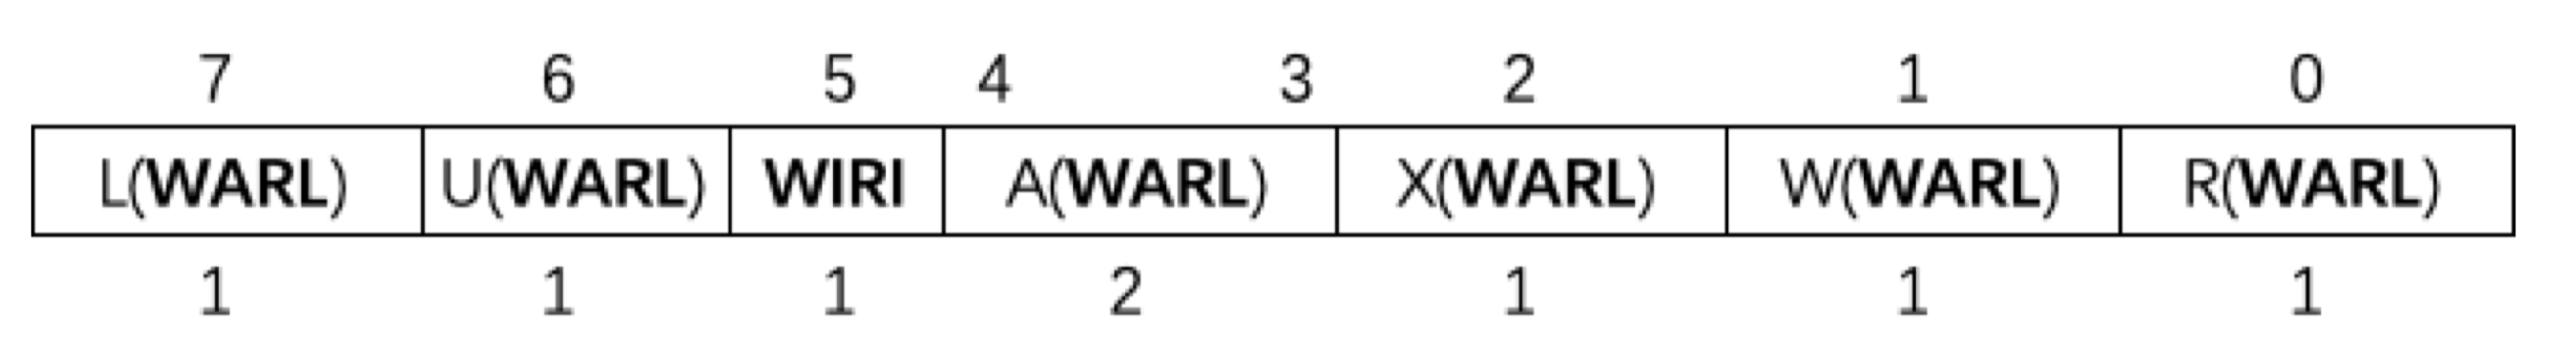
\includegraphics[scale=0.30]{Figures/extend/cfgformat.png}
    \decoRule
    \caption{CFG格式}
    \label{fig:cfgformat}
\end{figure}
\begin{figure}
    \centering
    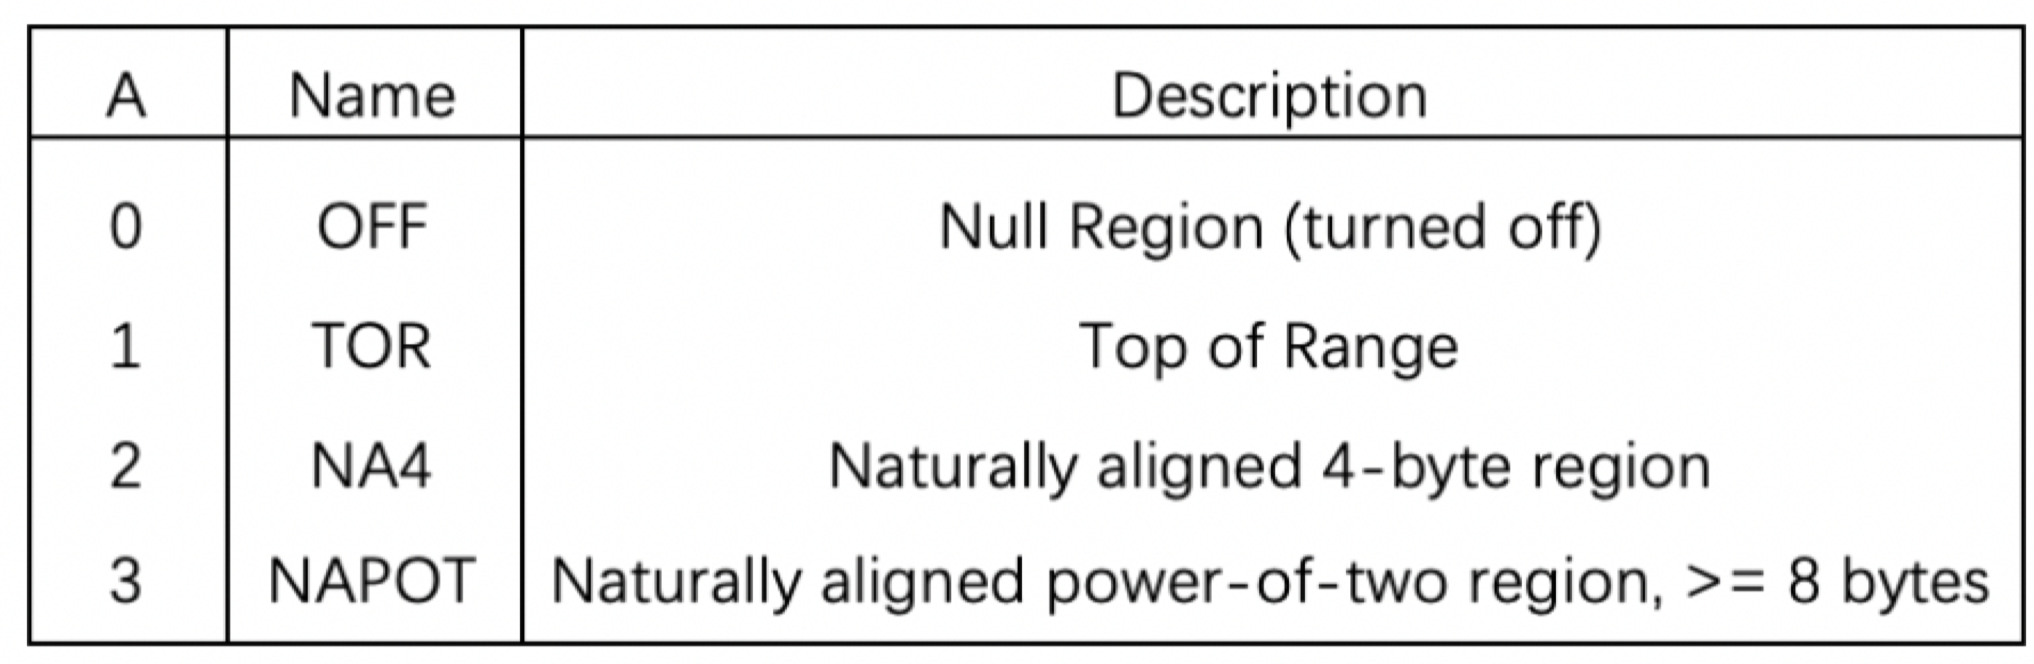
\includegraphics[scale=0.40]{Figures/extend/afield.png}
    \decoRule
    \caption{A位取值}
    \label{fig:afield}
\end{figure}
\begin{figure}
    \centering
    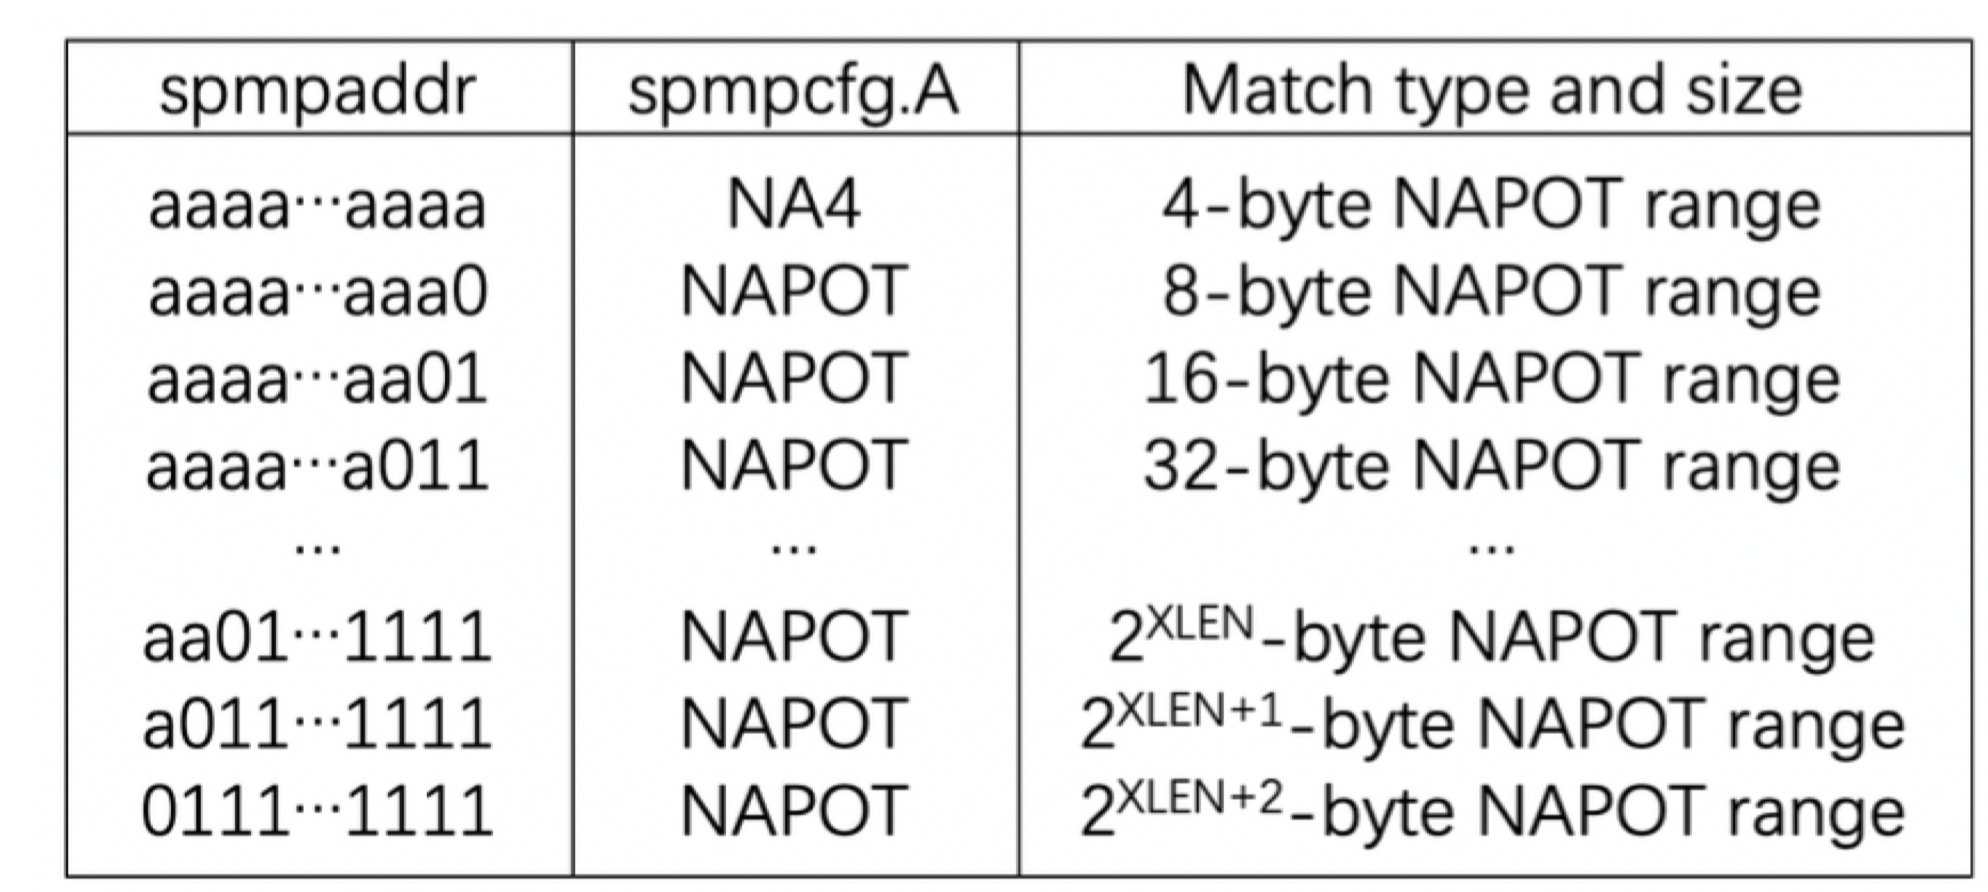
\includegraphics[scale=0.40]{Figures/extend/address.png}
    \decoRule
    \caption{地址空间划分}
    \label{fig:address}
\end{figure}

\subsection{权限和异常}
扩展的PMP只会在寻址已经通过了原来PMP的检查之后才会进行。
原始的PMP会通过最低位表示一次访问存储的成功或者失败。
首先PMP会检测其访问的地址是否在访问范围内,如果在不在访问范围内,则直接将结果设置为失败。
若在访问范围内,则根据实际的读写执行权限进行判定。
若访问失败,则会出现一个指令访问异常。
和原始PMP类似扩展的PMP也使用最低位来表示访存的失败,在原来PMP的检查之后,U模式下仍然会先检查方寸是否在扩展PMP规定的范围内,
这次检查相比于原始PMP的检查具有更细的粒度。在检查通过之后,仍然会根据读写执行权限进行判定,
若访问失败,会产生出一个页错误,这个错误可以交给U模式下kernel自己处理,也可以让更高层的Machine Code进行处理。


\section{场景分析}
\subsection{适用场景}
\subsection{不适用场景}

\section{小结} 
\chapter{总结} % Main chapter title

\label{Chapter6} % Change X to a consecutive number; for referencing this chapter elsewhere, use \ref{ChapterX}
本篇调研从题目出发,首先对ARM TrustZone,Intel SGX和RISC-V这一类硬件扩展及指令集进行了调研学习,列出了其基本设计思想和硬件实现思路
之后对于每一种特殊的硬件扩展,分别选用了一种Case进行样例研究,具体包括基于ARM TrustZone的SANCTUARY,基于Intel SGX的Graphene,基于
RISC-V的KeyStone设计。对于每一种Case,分别列出了威胁模型,保证的安全性质和能够防御的一些具体攻击,分析了具体设计的性能,
可扩展性和不足之处。

对于基于ARM TrustZone的SANCTUARY,除了给出了具体的分析之外,还列出了不适合SANCTUARY使用的具体场景,并对其不能支持多线程的问题在
视频渲染场景下的性能开销问题进行具体分析。对于基于RISC-V的KeyStone设计,我们在PMP方案原本的基础上,提出了基于PMP隔离不充分的问题,给出扩展方案来优化在上述分析中的不足点。主要解决了PMP寄存器
数量较少和在IoT场景中,没有页表情况下,只有PMP隔离不充足的问题。最后给出了具体的场景分析,来说设计的实用性。

总结来说系统安全的重要性随着人们越来越多的使用计算资源和依赖系统平台而变得越来越重要,而很多单纯依靠软件解决的安全问题主要
将面临威胁解决不彻底等问题,其本质也是性能与安全性的折衷,很大程度上牺牲了性能,很多设计具有安全性,但是一定程度上不具有可用性。
而硬件的解决方案,虽然有性能上的优势,但是由于是固件很难具有通用性。
在如今如数字版权保护,个人隐私保护,数据加密安全等方面都需要系统安全措施,所以基于硬件辅助和软件扩展的安全解决方案也必将成为主流。 


%----------------------------------------------------------------------------------------
%	THESIS CONTENT - APPENDICES
%----------------------------------------------------------------------------------------

%\appendix % Cue to tell LaTeX that the following "chapters" are Appendices

% Include the appendices of the thesis as separate files from the Appendices folder
% Uncomment the lines as you write the Appendices

%\include{Appendices/AppendixA}
%\include{Appendices/AppendixB}
%\include{Appendices/AppendixC}

%----------------------------------------------------------------------------------------
%	BIBLIOGRAPHY
%----------------------------------------------------------------------------------------

\renewcommand{\bibname}{参考文献}
\printbibliography[heading=bibintoc]

%----------------------------------------------------------------------------------------

\end{document}  
